\documentclass[4pt]{article}
\usepackage{pdflscape}
\usepackage[margin=0.2in,top=0.1in,bottom=0.1in]{geometry}
\usepackage{multicol}
\usepackage{parskip}
\usepackage{titlesec}
\titlespacing*{\subsubsection}{0pt}{10pt}{*0}

\usepackage{amsmath}
\usepackage{amssymb}
\usepackage{amsthm}
\usepackage{siunitx}
\usepackage{esint}
\usepackage{hanging}
\usepackage{xfrac}
\usepackage{tikz}
\usetikzlibrary{positioning}
\pagenumbering{gobble}


\theoremstyle{definition}
\newtheorem*{claim}{Claim}
\theoremstyle{definition}
\newtheorem*{lemma}{Lemma}
\renewcommand{\qed}{\hfill\blacksquare}
\renewcommand{\c}{\mathrm{c}\,}
\newcommand{\s}{\mathrm{s}\,}
\renewcommand{\r}{\mathrm{r}\,}             % abbreviation for rect()
\renewcommand{\o}{\omega}
\newcommand{\ra}{\rightarrow}
\newcommand{\lra}{\leftrightarrow}
\newcommand{\ulint}{\int_{0^-}^{\infty}}    % Unilateral Lt INTegral
\DeclareMathOperator{\rect}{rect}
\DeclareMathOperator{\sinc}{sinc}
\DeclareMathOperator{\sgn}{sgn}



\newcolumntype{Y}{>{\centering\arraybackslash}X}
\setlength{\abovedisplayskip}{0pt} % Space above display math
\setlength{\belowdisplayskip}{0pt} % Space below display math
\setlength{\abovedisplayshortskip}{0pt} % Space above when preceded by a short line
\setlength{\belowdisplayshortskip}{0pt} % Space below when followed by a short line


\title{Signals and Systems Exam 3}
%\usepackage[left=1in,right=1in,top=1in,bottom=1in]{geometry} % Adjust page margins
\usepackage{fancyhdr} % For custom headers and footers

\begin{document}
\begin{landscape}
\raggedright
\begin{multicols}{3} % Use 3 columns
\raggedcolumns
%\section*{Foundation}
\subsubsection*{Algebra}
    $\arctan(\frac{1}{\sqrt{3}}) = \frac{\pi}{6}$,  $\arctan(\sqrt{3}) = \frac{\pi} 3$

    $\sin n\pi = 0$\\
    $1-\cos n\pi = 2$ for odd $n$

    $\sin(x\pm y) = \sin x \cos y \pm \cos x \sin y$\\
    $\cos(x\pm y) = \cos x \cos y \mp \sin x \sin y$

    $\sin x \sin y = \sfrac{1}{2}[\cos(x-y) - \cos(x+y)]$\\ % annotate for sin 2x and cos 2x
    $\cos x \cos y = \sfrac{1}{2}[\cos(x-y) + \cos(x+y)]$\\
    $\sin x \cos y = \sfrac{1}{2}[\sin(x-y) + \sin(x+y)]$

    $C \cos(\o_0 t + \theta) = C\cos(\theta) \cos(\o_0 t) - C\sin(\o_0)\sin(\o_0 t)$\\        % highlight minus in cosine
    $C \sin(\o_0 t + \theta) = C\sin(\theta) \cos(\o_0 t) + C\cos(\o_0)\sin(\o_0 t)$

    $\theta = \tan^{-1} (-b/a)$, $\pm \pi$ when $a<0$\\
    $\sin t = \cos (t-\pi/2)$

    $\cos x = \frac{1}{2}\,[e^{jx} + e^{-jx}]$\\
    $\sin x = \frac{1}{2j}\, [e^{jx} - e^{-jx}]$\\
    $e^{j\o t} = \cos(\o t) + j\sin (\o t)$

    $z^* = a-jb = re^{-j\theta}$\\
    $u^* v^* = (uv)^*$

    $\angle z = \tan^{-1}(b/a)$, $\pm \pi$ in Q2 and Q3

    $z^{\frac 1 n} = r^{\frac 1 n} e^{j \frac{\theta + 2\pi m}{n}}$

    \((s+a)(s+b)(s+c) = s^3 + (a+b+c) s^2 + (ab+bc+ca)s + abc\)
%\rule{\linewidth}{0.5pt}
\subsubsection*{Integrals}
    % For sin, swap all explicit + with - and swap all cos with sin
    $\int \cos^2 at \, dt = \frac{t}{2} + \frac{\sin2at}{4a}$

    $\int t \cos at \, dt = \frac{1}{a^2}(\cos at + at\sin at)$\\
    $\int t^2 \cos at\, dt = \frac{1}{a^3}(2at\cos at - 2\sin at + a^2t^2\sin at)$

    $\int te^{at}\, dt = \frac{1}{a^2} \, e^{at} (at-1)$\\
    $\int t^2 e^{at} \, dt = \frac{1}{a^3} \, e^{at} (a^2t^2 - 2at + 2)$

    $\int e^{at} \,\cos bt \, dt = \frac{1}{a^2+b^2} \,e^{at}(a\cos 
    bt + b \sin bt)$

    \(\int \frac{1} {x^2+a^2}\, dx = \frac{1}{a} \tan^{-1} \frac x a\)

    \(
        \setlength{\jot}{0pt} % reduce the space between lines
\begin{aligned}
    a &= b + c \\
    x &= y + z \\
    p &= q + r
\end{aligned}
\)


\columnbreak
\subsubsection*{Signals}
    $\mathcal{E}_f = \int_{-\infty}^{\infty} |f(t)|^2 dt$ (complex); \\
    $P_f = \lim_{T\ra\infty}\frac{1}{T} \int^{T/2}_{-T/2} |f(t)|^2 dt $; \\
    rms power $= \sqrt {P_f}$

    % can't be both energy/power
    Cont; 
    analog; 
    periodic (extension); 
    (non/anti)causal; 
    energy/power (both); 
    deterministic/stochastic (info)

    $\int f(t)\cdot \delta(t - t_0) dt = f(t_0)$ ($f$ cont at $t_0$)
    

    out--in  $f(2x-6)$: shift by 6, scale by 2; $f(2(x-6))$: scale by 2, shift by 6

    $f_e(t) = \sfrac{1}{2}[f(t) + f(-t)]$; \\
    $f_o(t) = \sfrac{1}{2}[f(t) - f(-t)]$
\subsubsection*{Systems}
    L: $\mathcal{T}[kf_1(t) + f_2(t)] = ky_1(t) + y_2(t)$.\\
    $\mathcal{T}$: $\sum_{k=0}a_k D^k \, y(t) = \sum_{l=0}b_lD^l\, f(t)$,\\
    L if $a_k$, $b_l$ are not functions of $y(t), f(t)$\\
    E. $\sin\dot{y}(t) + t^2 y(t) = (t+3) f(t)$
    
    TI: $\mathcal{T}[f(t-\tau)] = y(t-\tau)$.\\
    $a_k$, $b_l$ indep of $t$. (const coeff)\\
    Let $g(t)\equiv f(t-\tau)$, find $z(t) = \mathcal{T}[g(t)]$


    Causal: $y(t)$ dep only on $f(\tau)$, $\tau < t$. 
    Compare $t$ and $\tau$.
    
    Ins/dyn: $y$ only dep $f$ at present (no $\int$)
    
    Invertible: given $y(t)$, we can know $f(t)$
\subsubsection*{Conv prop}
    $c(t) \equiv \int_{-\infty}^{\infty} f(\tau) g(t-\tau) d\tau$

    $f * g = g * f$
    
    $f * (g + h) = f * h + g * h$
    
    $f * (g * h) = (f * g) * h$

        Pf: $f * (g * h) = f * (h * g) = \int f(\tau_1) \int h(\tau_2)\, g(t - \tau_1 - \tau_2) \, d\tau_2 \, d\tau_1$
    
     $f(t - T_1) * g(t - T_2) = c(t - T_1 - T_2)$

     $f(at) * g(at) = |\sfrac{1}{a}|\, c(at)$ (even/odd)

     $f^{(m)} (t) * g^{(n)} (t) = c^{(m+n)}(t)$


    Graph: shift LEFT by $t$, and reflect. Every $\tau$ replaced by $t-\tau$, reverted
\columnbreak
\subsubsection*{Conv table}
    $f(t) * \delta(t-T) = f(t-T)$
    
    $u(t) * u(t) = t \, u(t)$

    $e^{at} \,u(t)* \,u(t) = \frac{1-e^{at}}{-a}\, u(t)$

    % Watch the sign.
    $e^{at}\,u(t) * e^{bt}\,u(t) = \frac{e^{at} - e^{bt}}{a - b}\, u(t)$ ($te^{at} \, u(t)$) 

    $e^{at}\, u(t) * e^{bt} \,u(-t) = \frac{e^{at} \, u(t) + e^{bt} \, u(-t)}{b-a}$

    % + here
    $te^{at}\,u(t) * e^{at} \,u(t)= \sfrac{1}{2} \,t^2e^{at} \, u(t)$

    $t^m\, u(t) * t^n \, u(t) = \frac{m!n!}{(m+n+1)!}\, t^{m+n+1} \, u(t)$

    Don't forget $[u(t+T_1) - u(t-T_2)]$ term
\subsubsection*{Response}
    $Q(D) y(t) = P(D) f(t)$, typically $\int f$\\
    Assume causal input $f(t) u(t)$

    $y_{zs}(t) = f(t) * h(t)$ from input\\    
        $y_{zs}(0^-) = 0$, $y_{zs}(0^+) \neq 0$

        Let $h(t) = \mathcal{T} [\delta (t)]$ (impulse response)
        % More description here
            $y_{zs}(t)=\mathcal{T} [f(t)] = \mathcal{T} [f(t) * \delta (t)]$\\
            \hspace{2.75em}$=\mathcal{T}[\lim\sum f(n\Delta\tau) \delta(t - n\Delta\tau) \Delta\tau]$\\
            \hspace{2.75em}$=\lim\sum f(n\Delta\tau) h(t-n\Delta\tau)\Delta\tau = f * h$
            
        $y_{zi}(t)$ from ini, $f(t)=0$,
            $Q y_{zi}(t) = 0$;
            % same for the derivatives of y
            $y_{zi}(0^-) = y_{zi}(0^+)$, $\dot{y_{zi}}(0^-) = \dot{y_{zi}}(0^+)$
%\section{FS}
\subsubsection*{Ortho set}
    $\mathcal{E}_e = \int_{t_1}^{t_2} [e(t)]^2 dt$\\
    $= \int_{t_1}^{t_2} f^2(t)dt - 2\sum c_i \int_{t_1}^{t_2} f(t) x_i(t) dt + \int_{t_1}^{t_2} (\sum c_i x_i(t))^2 dt$\\
    $    = \mathcal{E}_f -  2\sum_{c_i} \langle f, x_i \rangle$\\
    \hspace{1em}$+(\sum c_i^2 \int_{t_1}^{t_2} x_i(t)^2 dt + \sum_{i\neq j} c_i c_j \int_{t_1}^{t_2} x_i(t) x_j(t) dt)$
        
    $\frac{\partial \mathcal{E}_e}{\partial c_i} = 0 = -2 \langle f(t), x_i(t)\rangle + 2\mathcal{E}_i c_i$\\
    $\mathcal{E}_e^{\text{min}} = \mathcal{E}_f - \sum_{i=1}^N c_i^2 \mathcal{E}_i$

    \(c_i = \frac{1}{\mathcal{E}_i}\langle f, x_i\rangle = \frac{\int f(t) x(t) dt}{\int x_i^2(t) dt}\)    

    For ortho, $E_z = E_x + E_y$
        

    $|u+v|^2 = |u|^2 + |v|^2 + u^*v + v^*u$

    $\langle x(t), y(t)\rangle = \int_{t_1}^{t_2} x(t) y(t)^* \, dt = \int_{t_1}^{t_2} x(t) y(t) dt$ if real\\
    Use prod $\ra$ sum identities
\newpage
\subsubsection*{FS}
%\vfill\null
%\columnbreak 
    $a_0 = \frac{1}{T_0} \int_{T_0} f(t)\, dt$\\
    $a_n = \frac{2}{T_0} \int_{T_0} f(t) \cos(n\o_0t)\,dt$\\
    $b_n = \frac{2}{T_0} \int_{T_0} f(t) \sin(n\o_0t)\,dt$\\
    Energy: $T_0$ for $n=0$; $T_0/2$ else
     
    Half-w sym: $f(t - \sfrac{T_0}{2}) = -f(t)$\\
    $a_{n_\mathrm{odd}} = \frac{4}{T_0}\int_{0}^{T_0/2} f(t) \cos (n\o_0 t) \, dt$

    $f(t) = \sum_{n=-\infty}^{\infty} F_n e^{jn\o_0 t}$\\
    $F_n = \frac{1}{T_0}\int_{T_0} f(t) e^{-jn\o_0t}\,dt$

    $C_n\cos(n\o_0 t + \theta_n) = \sfrac{C_n}{2} \, (e^{j(n\o_0t + \theta_n)} + e^{-j(n\o_0 t + \theta_n)})$\\
    $ \hspace{5em}= (\frac{C_n} 2 e^{j\theta_n}) e^{jn\o_0 t} + (\frac{C_n} 2 e^{-j\theta_n}) e^{-jn\o_0 t}$

    $F_n = \frac{C_n}{2}\, e^{j\theta_n} = \frac 1 2 (a_n - jb_n) = |F_n| e^{j\angle F_n}$\\
    $F_{-n} = \frac{C_n}{2}\, e^{-j\theta_n} - \frac 1 2 (a_n + jb_n)$  % highlight the + and -!!, opposite
\subsubsection*{Existence}
    W: finite $\int$, fin $a$, $b$, fin power

    S: fin m/m/dcont over $T_0$, $\ra \frac{f(t_0^+) + f(t_0^-)}{2}$
\subsubsection*{FS prop}
    Time shift: $f(t-t_0)\lra F_n e^{-jn(\o_0 t_0)}$, $|F_n|$ same, $\angle F_n$ shifted by $-(\o_0 t_0)n$

    Reversal: $f(-t)\lra F_{-n}$

    Scal: $T = \sfrac {T_0} a$, $\o = a\o_0$

    Multip (same $T_0$): $f(t) g(t) \lra F_n * G_n$ 
        $\frac 1{T_0}  \int_{T_0} f(t) g(t) e^{jn\o_0 t}\, dt$\\
        $ = \frac{1}{T_0} \int (\sum F_m e^{jm\o_0 t}) (\sum G_k e^{jk\o_0 t}) e^{-jn\o_0 t} \, dt$ \\
        $ = \sum_m \sum_k F_m G_k \frac{1}{T_0} \int_{T_0} e^{j(m+k-n)\o_0 t} \, dt$\\
        $ = \sum_m \sum_k F_m G_k \langle e^{j(m+k)\o_0 t}, e^{jn\o_0 t}\rangle$\\
        $ = \sum_{k=-\infty}^{\infty} G_k F_{n-k}$
        
    Conjugation: $f(t)^* = F^*_{-n}$

    Parseval (power): \(P_f = \frac 1{T_0}\int_{T_0} f(t) f(t)^* dt\)\\
    \(=\frac{1}{T_0}\int_{T_0} (\sum_n F_n e^{jn\o_0t})(\sum_m F_m e^{jm\o_0t})^* dt\)\\
    \(=\sum_n \sum_m  F_n F_m^* \, \frac{1}{T_0}\int_{T_0} e^{j(n-m)\o_0t} dt\)\\
    \(=\sum_n |F_n|^2 \cdot 1\)

        $f$ real $\ra$ $|F|$ even, $\angle F$ odd\\
        $f$ real, even $\ra$ $F$ re, e; $F_{-n} = F_n = F_n^*$\\
        $f$ re, od $\ra$ $F$ im, o; $-F_{-n} = F_n = -F_n^*$

        $f_e(t) \lra \mathrm{Re}\{ F_n\}$\\
        $f_o(t) \lra j \,\mathrm{Im} \{F_n\}$
\columnbreak
\subsubsection*{Common FS}
    Square ($A=1$, $T=2\pi$, $\omega = 1$) 
        $\frac{4}{\pi}(\cos t - \frac{1}{3}\cos 3t + \frac{1}{5} \cos 5t- ...)$\\
        $\frac{4}{\pi}(\sin t + \frac 1 3 \sin 3t + \frac 1 5 \sin 5t + ...)$

    Triangle: 
        $\frac{8}{\pi^2}(\sin t - \frac{1}{9} \sin 3t + \frac{1}{25} \sin 5t - ...)$\\
        $\frac{8}{\pi^2}(\cos t + \frac 1 9 \cos 3t + \frac 1 {25} \cos 5t + ...)$

    Sawtooth:   
        $\frac 2{\pi} (\sin t - \frac{1}{2} \sin 2t + \frac{1}{3} \sin 3t - ...)$\\
        $\frac 2{\pi} (-\sin t - \frac{1}{2} \sin 2t - \frac{1}{3} \sin 3t - ...)$

    $\delta$ train:     
        $\delta_{T_0} (t) = \sum_{n=-\infty}^{\infty} \delta(t - nT_0)$ \\
        $\frac{1}{T_0} \sum_{n=-\infty}^{\infty} e^{jn\omega_0 t}$

    % square duty cycle add here
%\section{FT}
\subsubsection*{FT}
    Let \(F(\omega) \equiv \int f(t) e^{-j\omega t} \, dt\)

    \(F_n = \frac 1 {T_0} \int_{T_0} f(t) e^{-jn\omega_0 t} \, dt\)

    Limit as $\omega_0 =\Delta\omega \ra 0$,\\
    \(F_n = \frac {\Delta\omega}{2\pi} \int f(t) e^{-jn\Delta\omega t} \, dt
    \equiv \frac{\Delta\omega}{2\pi} F(n\Delta\omega)\) % substitute t for n\Delta\omega

    \(f_{T_0}(t) = \sum F_n\, e^{jn\omega_0 t} = \sum \frac {\Delta\omega} {2\pi} F(n\Delta\omega)\,  e^{jn\Delta\omega t}\)

    % variable iof integration is \omega!
    % lim T0 -> infty
    % can also write delta \onega0/2pi = 1/T0
    % sum to integral
    \(f(t) = \lim f_{T_0} (t) = \frac{1}{2\pi}\int F(\omega) e^{jt\omega} d\omega\)

    \(F(\omega) = |F(\omega)| \, e^{j\angle F(\omega)}\)

    Re signals: sym of $||$ and $\angle$

    Existence: energy signal ($|e^{-j\o t}| = 1$)\\
    Strong: fin num max/min/discont

\subsubsection*{FT Table}

    \(\delta(t) \lra 1\)\\
    $1 \lra 2\pi\delta(\omega)$

    \(e^{j\o_0 t}\ra 2\pi\delta(\o - \o_0)\)\\         % inverse transform this, watch minus sign
    \(\cos \o_0 t\ra \pi[\delta(\o+\o_0) + \delta(\o - \o_0)]\)\\
    \(\sin \o_0 t\ra j\pi[\delta(\o + \o_0) - \delta(\o - \o_0)]\)

    \(\sum \delta(t-nT_0) \ra \o_0\sum \delta(\o - n\o_0)\)        % what is omega_0

    $e^{-at} \, u(t) \ra \frac{1}{a+j\omega}$\\         % a > 0
    $e^{-a|t|} \ra \frac{2a}{a^2+\omega^2}$ \\
    \(u(t) = \lim_{a\ra 0} e^{-at} u(t)\ra \lim \frac{1}{a+j\o}\)
    \( = \lim(\frac{a}{a^2+\o^2} - j\frac{\o}{a^2+\o^2 }) = \pi\delta(\o) + \frac{1}{j\o}\) \\      % acrtan integral to get pi
    \(\sgn(t)\ra \frac{2}{j\o}\)

    \(t^n e^{-at} u(t)\ra \frac{n!}{(a+j\o)^{n+1}}\)

    \(\cos \o_0 t\, u(t)\ra \frac{\pi}{2}(\delta(-) + \delta(+)) + \frac{j\o}{\o_0^2-\o^2}\)\\       % write out - and +
    \(\sin \o_0 t\, u(t)\ra \frac{\pi}{2j}(\delta(-) - \delta(+)) + \frac{\o_0}{\o_0^2-\o^2}\)\\
    \(e^{-at}\cos \o_0t\, u(t)\ra \frac{a+j\o}{(a+j\o)^2 + \o_0^2}\)\\
    \(e^{-at}\sin \o_0t\, u(t)\ra \frac{\o_0}{(a+j\o)^2 + \o_0^2}\)           


    % width \tau, draw a diagram
    $\rect(\frac t {\tau}) \ra \tau \sinc(\frac{\tau}{2}\omega)$\\ 
    $\frac W \pi \sinc(Wt) \ra \rect(\frac{\omega}{2W})$

    % draw a diagram as well
    \(\triangle (\frac t {\tau}) \ra \frac{\tau}{2} \sinc^2 (\frac{\tau}{4}\omega)\)\\
    \(\frac{W}{2\pi} \sinc^2 (\frac{W}{2}t) \ra \triangle(\frac{\omega}{2W})\)

    \([\o^2 \r(\frac{\o}{2\o_0})] \leftarrow \frac{1}{2\pi} \frac{e^{j\o t}}{(jt)^3}(-\o^2t^2-2j\o t + 2)^{\o_0}_{-\o_0}\)\\
    \(=\frac{(\o_0^2 t^2 - 2)\sin \o_0 t + 2\o_0 t\cos \o_0 t}{\pi t^3}\)\

    \([\frac{|\o|}{\o_0} \rect(\frac{\o}{2\o_0})] \leftarrow \frac{\cos \o_0 t + \o_0 t \sin \o_0 t - 1}{\o_0 \pi t^2}\)
   % \columnbreak
\subsubsection*{Frequency domain prop}
    Linearity

    Time shift: \(f(t-t_0) \ra F(\omega) e^{-jt_0\omega}\) \\ % highlight negative signS
    $|F|$ unchanged; $\angle F =- t_0\omega$, lin shift

    Freq shift: \(f(t) e^{j\omega_0 t} \ra F(\omega - \omega_0)\)  % watch sign, again

    Dual: \(f(t) \ra F(\omega)\), \(F(t) \ra 2\pi f(-\omega)\)\\ 
    Pf. \(f(t) = \frac 1 {2\pi} \int F(\lambda) e^{jt\lambda}\, d\lambda\)\\
    % highlight the -t here
    \(2\pi f(-t) = \int F(\lambda) e^{-tj\lambda}\, d\lambda = \mathcal{F}[F(\lambda)]\)

    Reversal: \(f(-t)\ra F(-\o)\)

    Scaling: \(f(at)\ra \frac{1}{|a|}F(\frac{\o}{a})\)   % compress in t, expand in omega

    Convolution: \(f*g \ra FG\), \(fg \ra \frac{1}{2\pi} F*G\)\\
    \(\mathcal F[f*g] = \int e^{-j\o t} \int f(\tau) g(t-\tau)d\tau dt\)\\
    \(\hspace{3.75em}=\int f(\tau) \mathcal F[g(t-\tau)]  d\tau \)\\
    \(\hspace{3.75em}= \int f(\tau) G(\o)e^{-j\o\tau}d\tau\)
    % highlight above for the other direction
    \( \frac{1}{2\pi} \mathcal{F}^{-1}[F * G] = (\frac{1}{2\pi})^2 \int e^{j\o t} \int F(\lambda) G(\o - \lambda) d\lambda d\o\)

    Diff: \(f^{(n)}(t) \ra (j\o)^nF(\o)\) (diff $e^{j\o t}$)    % highlight j\omega
    
    Int: \(\int_{-\infty}^t f(\tau)d\tau \ra \frac{1}{j\o}F(\o) + \pi F(0) \delta(\o)\)\\
    \(U(\o) = \lim \frac{1}{a+j\o} = \lim (\frac{a}{a^2+\o^2} - j\frac{\o}{a^2+\o^2}) \) \\
    \(= \pi\delta(\o) + \frac{1}{j\o}\) ($\int \frac{a}{\o^2+a^2}d\o = \tan^{-1}=\pi$)\\
    $\int = f(t) * u(t) \ra F(\o)U(\o)$

    Conjugation: \(f(t)^* \ra F(-\o)^*\)   % highlight negative

    Sym: Re $\ra$ $||$ e, $\angle$ o ($F(-\o) = F(\o)^*$);\\
    re, e $\ra$ re, e; re, o $\ra$ im, o

    $f$ even: \(F(\o) = 2\int_0^{\infty} f(t)\cos(\o t) dt\)\\
    $f$ odd: \(F(\o) = -2j\int_0^{\infty} f(t) \sin(\o t) dt\)
\newpage
\subsubsection*{Parseval}
    Psval: \(E_f = \int |f(t)|^2 dt = \frac{1}{2\pi} \int |F(\omega)|^2 d\o\)  for energy sig\\  % highlight 1/2pi, and square
    Pf: \(= \int f f^* dt = \int f(t)\mathcal F ^{-1}[F(-\o)^*]dt\)\\
    \(= \int f(t) \frac{1}{2\pi} \int F(-\o)^* e^{j\o t} d\o dt\)\\
    \(= \frac{1}{2\pi}\int f(t) \int F(\lambda)^* e^{-jt\lambda} d\lambda dt \)\\
    \(= \int dt d\lambda\)

    \(\Delta E_f = \frac{2}{2\pi}\int^{\o_2}_{\o_1} |F(\o)|^2 d\o\) % highlight 2 due to +/-

    Autocorrelation \(\psi_f(t) \equiv \int f(\tau)f(\tau-t)d\tau \ra |F(\o)|^2\)   % annotate for general case w/o abs
\subsubsection*{AM}
    \(m(t) \cos(\o_c t) \ra \frac{1}{2}[M(\o + \o_c) + M(\o - \o_c)]\)\\     % highlight M, may be a factor of pi
    \(e(t) = m(t)\cos^2 \o_c t\)  \\          % highlight ^2
    \(E(\o) = \frac{1}{2} M + \frac{1}{4}[M(\o + 2\o_c) + M(\o - 2\o_c)]\)

    SSB: $1/4$ gain

    \(\phi_\mathrm{AM} (t) = [A + f(t)] \cos (\omega_0 t)\)\\
    $A \geq f(t)$ for all $t$

    modulation index \(\mu\equiv f_{\text{max}}/A\)\\
    $\mu = \infty$, SC, $\mu = 1$, marginal
\subsubsection*{LTIC sys trans, (m) stable}
    % p243
    Let \(e^{j\o t} \Rightarrow H(\o) e^{j\o t}\)

    % left side is f(t), right side is response y(t)
    \(\lim\sum \frac{F(n\Delta\o)\Delta\o}{2\pi} e^{jn\Delta\o t}\Rightarrow \lim\sum \frac{F(n\Delta\o)H(n\Delta\o)\Delta\o}{2\pi} e^{jn\Delta\o t}\)\\
    \(y(t) = \frac{1}{2\pi}\int F(\o)H(\o)e^{j\o t} d\o\)

    \(Y(\o) = F(\o) H(\o)\)

    Distortionless: $y(t) = kf(t-t_d)$,
    so $H(\o) = ke^{-j\o t_d}$          % highlight omega t_d, phase is equally important

    Payley-Wiener: $H$ realizable, $h$ causal iff \(\int\frac{|\ln|H(\omega)||}{1+\o^2} d\o < \infty\) (consecutive 0s)\\
    \(\hat{h}(t) = h(t) u(t)\)

\subsubsection*{Periodic FT}
    \(f(t) = \sum_n F_n e^{jn\o_0 t}\), \(\mathcal{F}[f(t)] = 2\pi \sum_n F_n \delta(\omega - n\o_0)\)      % highlight n!

    \(Y = F(\omega)H(\omega) = 2\pi \sum F_n H(n\omega_0) \delta(\omega - n\omega_0) \) \\            % due to delta
    $Y_n \equiv F_n H(n\o_0)$. Periodic with same $\omega_0$

    Eigen: $f(t) = e^{j\o_0t}$, \(Y_1 = H(1\o_0)\), $y(t) = H(1\o_0) e^{j\o_0 t}$

    $f(t) = \cos(\o_0 t + \theta)$, assume $h(t)$ real\\
    \(y = \frac 1 2 (e^{j(\theta + \o_0 t)}H(\o_0) + e^{-j(\theta + \o_0 t)}H(-\o_0))\)\\          % highlight -\omega_0
    \(=|H(\o_0)| \cos(\o_0t + \theta + \angle H(\o_0))\)

    \(\cos 2t * e^{-3t}\, u(t) \equiv f * h\)\\       % highlight 2 in both lines
    \(=|H(2)| \cos(2t + \angle H(2))\)              % you can just directly shift on the angle of trig
\columnbreak
\subsubsection*{Sampling}
    \(\overline{f}(t)\equiv f(t) \delta_{T_s}(t) = \sum f(nT_s) \delta(t - nT_s)\)\\
    % highlight 1/T_s, don't forget this term!
    \(\overline{F}(\o) = \frac{1}{2\pi} F(\o) * [\frac{2\pi}{T_s} \sum\delta(\o - n\o_s)]\)
    \(= \frac{1}{T_s}\sum F(\o - n\o_s)\)

    $\o_s \geq 4\pi B$, $F_s \geq 2B$

    \(F(\o) = \overline{F}(\o) T_s \rect(\frac{\o}{4\pi B})\)\\   % highlight T_s
    If $F_s = 2B$, \(f(t) = \overline{f}(t) * \frac{2B}{F_s} \sinc(2\pi Bt)\)\\       % cancel 2B, highlight the condition
    \(=\sum f(nT_s)\delta(t - nT_s) * \sinc(2\pi B t)\)
    \(= \sum f(nT_s) \sinc(2\pi Bt - n\pi)\)\\
    ana FS, basis: $\sinc$, interpolation formula

    If $F_s > 2B$, \(f(t) = \sum f(nT_s) w(t - nT_s)\)\\
    for some relaxed LP filter $w(t)$

    Anti-alias before sampling: LPF of $F_s/2$

    Practical sampling: \(p_T(t) = \frac{\tau}{T_s} + \sum(\frac{2}{\pi n}\sin(n\pi\frac{\tau}{T_s}))\cos(n\omega_s t)\)\\
    \(P_T(\o) = 2\pi \frac{\tau}{T_s}\delta(\o)\)
    \(+ \sum\frac{2\sin(...)}{n}[\delta(\o + n\o_s) + \delta(\o - n\o_s)]\)       % highlight first term
%\section{LT}
\subsubsection*{LT}
\(\mathcal L [-e^{-at}u(-t)] = \mathcal L [e^{-at} u(t)]\), except ROC\\
If sig are causal, $\mathcal L$ is 1-to-1           % highlight causal

Unilateral: \(\mathcal{L}[f] = \ulint f(t) e^{-st} dt\)\\          % highlight 0-, for unilateral
\(= \int [f(t) e^{-\sigma t}] e^{-j\o t} dt\)


$\sigma_0$: smallest $\sigma$ to make converge
\subsubsection*{Uni LT Table}
    Watch ROC!!     % highlight

    $\delta(t) \ra 1$ \hfill $\forall s$\\
    $u(t) \ra \frac{1}{s}$\hfill $\Re(s) > 0$\\
    $t^n u(t) \ra \frac{n!}{s^{n+1}}$               % highlight the u(t), also for e^t as well

    \(e^{\lambda t} u(t) \ra \frac{1}{s-\lambda}\) \hfill $\Re(s) > \Re(\lambda)$\\        % highlight -
    \(t^n e^{\lambda t} u(t) \ra \frac{n!}{(s-\lambda)^{n+1}}\)\\     % highlight +1
    \(\frac{1}{(n-1)!} t^{n-1} e^{\lambda t} u(t) \ra \frac{1}{(s-\lambda)^n} \)        % highlight -1, just inverse of the above
    % also highlight factorial!

    \(e^{-at} \cos bt\, u(t) \ra \frac{s+a}{(s+a)^2 + b^2}\)\\
    \(e^{-at} \sin bt\, u(t) \ra \frac{b}{(s+a)^2 + b^2}\)    

    %highlight minus sign. Check this. I'm not sure
    \(re^{-at} \cos(bt + \theta) u(t) \ra \frac{(r\cos\theta)s + (ar \cos\theta - br\sin \theta)}{s^2 + 2as + (a^2 + b^2)}\)\\
    % highlight 2
    \(2re^{-at} \cos(bt + \theta) u(t) \ra \frac{re^{j\theta}}{s-(-a+jb)}+\frac{re^{-j\theta}}{s-(-a-jb)}\)\\
    \(e^{-at}\left[A\cos(b t) + \frac{B-Aa}{b}\sin(bt)\right] u(t)\)\\
    \(\hfill \frac{\sqrt{A^2c + B^2 - 2ABa}}{b}e^{-at}\cos\left(bt + \tan^{-1}\frac{Aa-B}{Ab}\right) u(t)\)\\
    \(\hfill \ra \frac{As+B}{s^2+2as+c}\)
\columnbreak
\subsubsection*{LT Prop}
    Linearity \hfill ROC $\cap$\\
    Time delay \(f(t-t_0) u(t-t_0) \ra F(s) e^{-st_0}\)  \hfill same ROC\\    % t0 > 0 for causal
        $t_0 > 0$; Pf: \(\int_{-t_0}^{\infty}\)\\ % highlight -t0, and negative signs
    % also highlight t0 in u
    Freq shift \(f(t) e^{s_0 t} \ra F(s-s_0)\) ($\Re(s) > \sigma_0 + \Re(s_0)$)\\
    Scaling ($a > 0$), \(f(at) \ra \frac{1}{|a|} F(\frac{s}{a})\) ($\Re(s) > a\sigma_0 $)\\   % highlight a
    % a > 0 for causal, may not need abs
    Convolution \(f_1 * f_2 \ra F_1 F_2\) \hfill ROC $\cap$\\
    \(f_1 f_2 \ra \frac{1}{2\pi j} F_1 * F_2\)

    Time diff \(\dot{f}(t) \ra sF(s) - f(0^-)\) \hfill $\Re(s) > \max(\sigma_0, 0)$\\     % highlight s before F and -
        Pf (parts): \(\ulint \dot{f}(t) e^{-st} dt = \left[f(t) e^{-st} \right]^{\infty}_{0^-} + s F(s)\)\\    % highlight s again
    \(\ddot{f}(t) \ra s^2 F(s) - sf(0^-) - \dot{f}(0^-)\)   % highlight fdot, and minus signs
    % When used to LT piecewise functions, remember f(0-) = 0, f'(0-) = 0

    Time int \(\ulint f(\tau) d\tau \ra \frac{1}{s} F(s)\) Pf: diff     % highlight 0-, initial condition related

    Freq diff \(-t f(t) \ra \frac{dF(s)}{ds}\)          % highlight negative

    Freq int \(\frac{1}{t}f(t) \ra \int_s^{\infty}F(z) dz\)

    IVT \(f(0^+) = \lim_{s\ra \infty} sF(s)\) if exists\\
        Pf: \(\mathcal L[\dot{f} (t)] = \ulint \dot f(t) e^{-st} dt\)\\ % highlight dot
        \(sF(s) - f(0^-) = \int_{0^-}^{0^+} \dot f (t) e^{-st} dt + \int _{0^+}^{\infty} \dot f(t) e^{-st} dt \)\\    % last term goes away as s -> \inf
        \(sF(s) - f(0^-) = f(0^+) - f(0^-)\)    % cancel f0-

    FVT \(f(\infty) = \lim_{s\ra 0} sF(s)\) if exists\\
        Pf: \(\mathcal L[\dot{f} (t)] = \ulint \dot f(t) e^{-st} dt\)\\ % highlight dot, can delete this line
        \(\lim_{s\ra 0} sF(s) - f(0^-) = \lim_{s\ra 0}\ulint \dot f (t) e^{-st} dt\)\\    % e^-st = 1
        \(sF(s) - f(0^-) = f(\infty) - f(0^-)\)    % cancel f0-
\subsubsection*{Rational $\mathcal L^{-1}$}
    First make it rational      % highlight this!

    \(F(s) = \frac{b_ms^m + ... + b_1s + b_0}{s^n + ... + a_1s + a_0} \equiv \frac{P(s)}{Q(s)}\)

    \(k = (s-\lambda_i) F(s) | _{s = \lambda_i}\)

    % highlight ^r in both cases, and m
    \(a_0 = (s-\lambda)^r F(s)|_{s=\lambda}\)\\
    \(a_m = \frac{1}{m!} \frac{d^m}{ds^m}[(s-\lambda)^r F(s)] |_{s = \lambda}\)

    Multiply both by $s$ and let $s=\infty$, only $\frac{1}{s}$ term kept 
%\end{multicols}  
\newpage
\subsubsection*{Sys Anal}
    \(Q(D) y(t) = P(D) f(t)\)\\
    $H(s) = \frac{Y_{zs}(s)}{F(s)} = \frac{P(s)}{Q(s)}$  % highlight order, P/Q, not Q/P; highlight zs

    Asym. $(y_{zi} (t)$ dies out)\\         % highlight zi
    stable: $y_{zi}(t) \ra 0$ as $t\ra \infty$\\
    marginal: $y_{zi}(t)$ remains bounded (unrep $\lambda$ on Im axis)B

    BIBO iff \(\int_{-\infty}^{\infty} |h(t)| dt\) exists\\ % highlight abs
    $\Rightarrow$ $|f(t)| < K$\\                       % highlight zs
    \(\hspace{1.25em}y_{zs}(t) = h * f= \int h(\tau) f(t-\tau) d\tau\)\\
    \(\hspace{4em} \leq \int |h||f| d\tau < K \int |h(\tau)| d\tau\)\\
    $\Leftarrow$ Let $f(t) = \sgn(h(-t))$\\                % contrapositive
    \(\hspace{1.25em} y(0) = \int h(\tau) f(0-\tau) d\tau\)\\
    \(\hspace{3.25em} = \int h(\tau) \sgn(h(\tau)) d\tau\)\\
    \(\hspace{3.25em} = \int |h(\tau)| d\tau \equiv \infty\)

    Asy $\rightarrow$ BIBO st (all exp)\\                                % not the other way
    Marginal $\rightarrow$ BIBO ust ($\int |\sin|$)                            % cross BIBO
    % counterexample? pole and zero cancel??

\subsubsection*{Sys Realization}         % draw a diagraom for that
    % generally, m <= n
    % show realization of simple 1/(s+l)
    Feedback: \(Y = GE = G(F - HGY)\)\\
    \(H_{\text{eff}} = \frac{Y} F = \frac G {1+HG}\)

    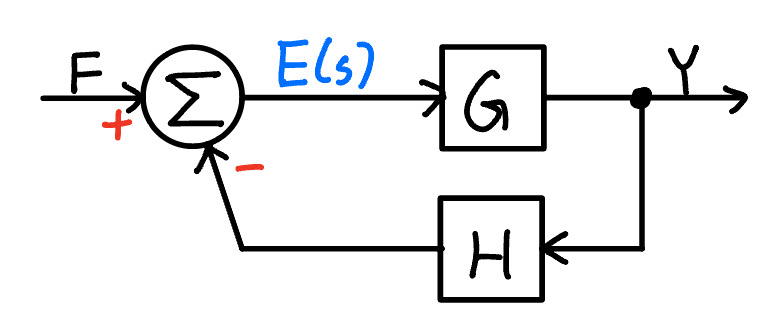
\includegraphics[width=0.5\linewidth]{figures/feedback.jpg}


    Canonical:\\              % diagram
    % m < n here!
    Always make $a_n = 1$\\
    \(F = s^2 X + a_1 sX + a_0 X\)\\
    \(s^2 X = F - a_1 sX - a_0 X\)      % highlight minus

    \(b_2 s^2 X + b_1 sX + b_0 X = Y\)

    % can you save a few summers for the parallel cases?

    \(H = \frac{b_1s+b_0}{1s^3+a_2s^2+a_1s+a_0}\)\\     % highlight 1 s^3

    \(
    \begin{bmatrix}
        \dot{x}_1\\
        \dot{x}_2\\
        \dot{x}_3\\
    \end{bmatrix}
    =
    \begin{bmatrix}
        0 & 1 & 0\\
        0 & 0 & 1\\
        -a_0 & -a_1 & -a_2      % highlight diagonal pattern
    \end{bmatrix}
    \begin{bmatrix}
        x_1\\
        x_2\\
        x_3
    \end{bmatrix}
    +
    \begin{bmatrix}
        0\\0\\1         % always 0 0 1
    \end{bmatrix}
    f
    \)\\

    \(y =
    \begin{bmatrix}
        b_0 & b_1 & 0      % b_0, b_1, ..., b_m, 0, ..., 0
    \end{bmatrix}
    \cdot \mathbf x
    \)\\
    Second form: \(s^2 Y = s^2 b_2 F + s(-a_1 Y + b_1 F) + (-a_o Y + b_0 F)\)\\
    \(Y = b_2 F + \frac 1 s(-a_1 Y + b_1 F) + \frac 1 {s^2}(-a_o Y + b_0 F)\)\\
    Transpose $A$, swap $\mathbf b$, $\mathbf c$

    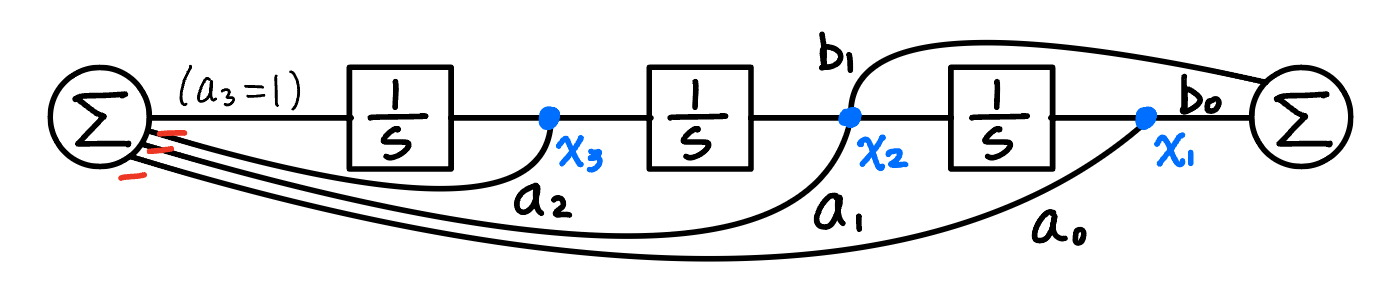
\includegraphics[width=\linewidth]{figures/canonical.jpg}
    Cascade:\\
    Make complication in the center\\
    \(H = \frac {P_1}{s+\lambda_1} \cdot \frac{P_2}{s+\lambda_2} \cdot \frac{k_3}{s+\lambda_3}\)\\
    \(
    \begin{bmatrix}
        \dot{x}_1\\
        \dot{x}_2\\
        \dot{x}_3\\
    \end{bmatrix}
    =
    \begin{bmatrix}
        -\lambda_1 & 0 & 0\\
        .. & -\lambda_2 & 0\\
        .. & .. & -\lambda_3\\     % highlight lower triangular
    \end{bmatrix}
    \begin{bmatrix}
        x_1\\
        x_2\\
        x_3
    \end{bmatrix}
    +
    \begin{bmatrix}
        1\\..\\..         % always 1 x x
    \end{bmatrix}
    f
    \)\\

    \(y =
    \begin{bmatrix}
        .. & .. & k_3       % always x x 1
    \end{bmatrix}
    \cdot \mathbf x
    \)
    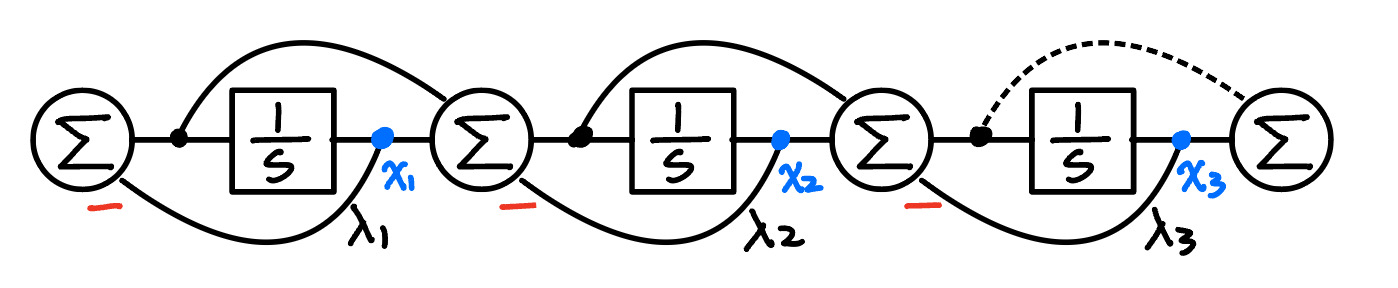
\includegraphics[width=\linewidth]{figures/cascade.jpg}

    Parallel:\\
    \(H = \frac{k_1}{s+\lambda_1} + \frac{k_2}{s+\lambda_2} + \frac{k_3}{s+\lambda_3}\)\\
    \(
    \begin{bmatrix}
        \dot{x}_1\\
        \dot{x}_2\\
        \dot{x}_3\\
    \end{bmatrix}
    =
    \begin{bmatrix}
        -\lambda_1 & 0 & 0\\
        0 & -\lambda_2 & 0\\
        0 & 0 & -\lambda_3\\    % highlight diagonal
    \end{bmatrix}
    \begin{bmatrix}
        x_1\\
        x_2\\
        x_3
    \end{bmatrix}
    +
    \begin{bmatrix}
        1\\1\\1         % always 1 1 1
    \end{bmatrix}
    f
    \)\\

    \(y =
    \begin{bmatrix}
        k_1 & k_2 & k_3       % k_1, ..., k_n
    \end{bmatrix}
    \cdot \mathbf x
    \)
    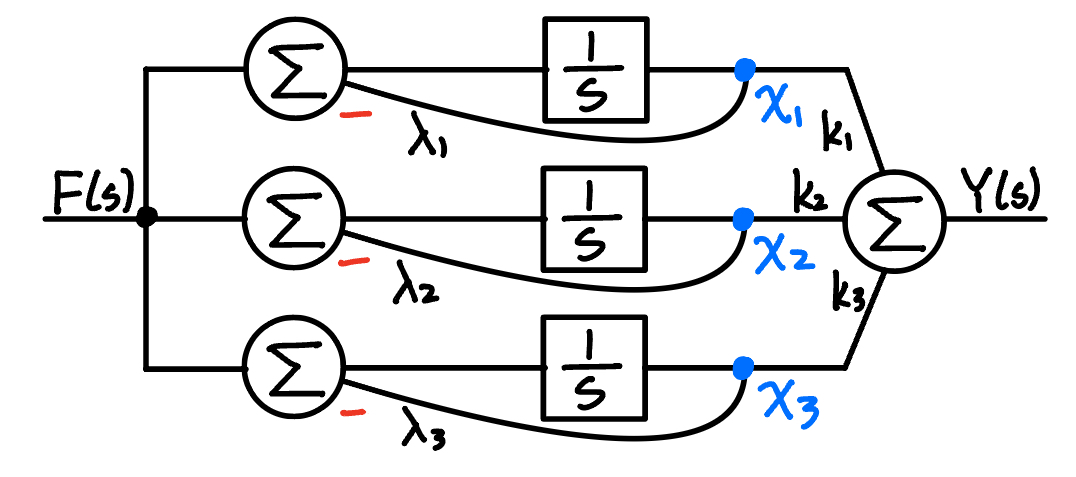
\includegraphics[width=0.75\linewidth]{figures/parallel.jpg}


    Same pole                           % diagram for that, draw s-domain first, and then fully realize
    \(H = \frac{a_0}{(s-\lambda)^2} + \frac{a_1}{s-\lambda} + \frac{k_1}{s-\alpha_1}\)      % highlight ^2
    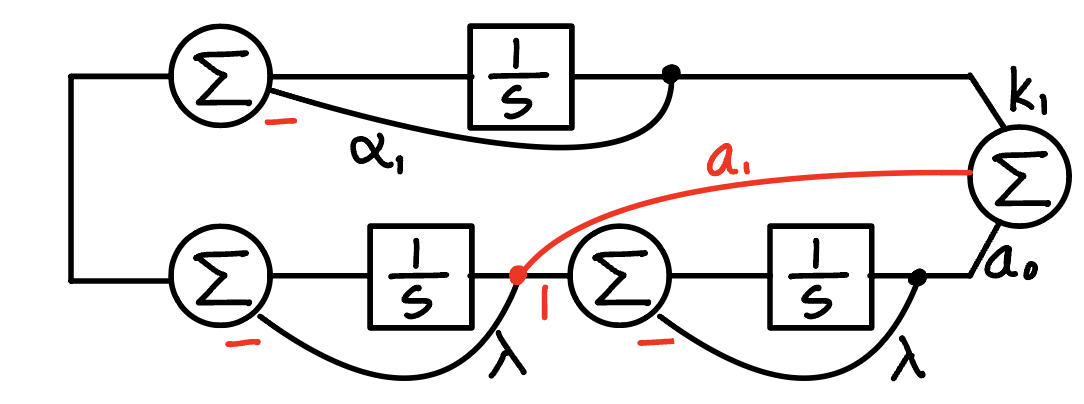
\includegraphics[width=0.7\linewidth]{figures/multipole.jpg}

\columnbreak
\subsubsection*{State Equations}
    Def: state at any time $t_0$: smallest set of nums $\{x_i(t_0)\}$ that is sufficient to detemrine sys behavior $\forall t > t_0$ for given input $f$\\
    Initial condition if $t_0 = 0$

    Always int. output

    \(\mathbf{\dot x} = A \mathbf x + \mathbf b f\)\\
    \(y = \mathbf{c} \cdot \mathbf x\)

    Multiple i/o:
    \(\mathbf{\dot x} = A \mathbf x + \mathbf B \mathbf f\)\\
    \(\mathbf y = \mathbf C \mathbf x + \mathbf D \mathbf f\)

    \(s \mathbf X(s) - \mathbf x(0) = A \mathbf X(s) + \mathbf B \mathbf F(s)\)\\
    \((s \mathbf I - \mathbf A) \mathbf X(s) = \mathbf x(0) + \mathbf B \mathbf F(s)\)\\
    \(\mathbf X(s) = (s \mathbf I - \mathbf A)^{-1} \mathbf x(0) + (s \mathbf I - \mathbf A)^{-1} \mathbf B \mathbf F(s)\)\\
    % zero input and zero state
    substitute $\mathbf X$ for $\mathbf Y_{zi}$ and $\mathbf Y_{zs}$
    



\subsubsection*{Frequency Response}
    \(H(\o) = H(s)|_{s = j\o}\) % first H is F, second is L

    % highlight abs
    Ideal delay: \(|H| = 1, \angle(\o) = -\o T\)\\      % comes from exp(j..)
    Ideal diff: \(|H(\o)| = |\o|, \angle H = \pm\frac {\pi} 2\)\\
    Ideal int: \(|H(\o)| = \frac 1 {|\o|}\), \(\angle H = \mp \frac{\pi} 2\)
    % symmetry for -omega

    \(f(t) = e^{j\o_0 t}\, u(t)\) thru \(H(s) = \frac{P(s)}{Q(s)}\)\\   % highlight j and u(t)
    \(Y_{zs}(s) = F(s) H(s)\)\\      % highlight zs!!
    \(= \frac 1 {s - j\o_0} \frac{P(s)}{(s-\lambda_1)...(s-\lambda_n)}\)\\
    \(= \frac{H(s)|_{s=j\o_0}}{s-j\o_0} + \frac{k_1}{s-\lambda_1} ...\)\\
    \(y_{zs}(t) = H(\o_0)  e^{j\o_0 t} \, u(t) + \sum_i k_i e^{\lambda_i t} \, u(t)\)
    % highlight u(t) on the last step, and zero state "zs"

    $y_{ss}(t)$ scaled input\\
    $y_{tr}(t)$ decays for stable sys

    \(f(t) = \cos(\o_0 t + \theta) \, u(t)\)\\
    \(y_{ss}(t) = |H(\o_0)| \cos(\o_0 t + \theta + \angle H(\o_0)) u(t)\)
    % highlight ss and u(t)

\subsubsection*{Filter Design}
    \(H(j\o) = b_n \frac{(j\o-z_1)..(j\o-z_n)}{(j\o-p_1)..(j\o-p_n)}\)\\\
    \(= b_n \frac{(r_1 e^{j\phi_1})...(r_n e^{j\phi_n})}{(d_1 e^{j\theta_1})... (d_n e^{j\theta_n})}\)\\
    \(|H(j\o)| = b_n \frac{r_1 ... r_n}{d_1 ... d_n}\)\\
    \(\angle H(j\o) = (\phi_1 + .. + \phi_n) - (\theta_1 + .. + \theta_n)\)\\
    % give a graphical example
    % example of z = -1, p = -2 may be useful

    Vector from p/z to $j\o$
    % pole enhances gain, zero suppresses.
\end{multicols}
\end{landscape}
\end{document}
